\vspace{-.1in}
\section{Use Cases}
\label{sec:use_cases}

\subsection{Combustion}
\label{sec:combustion}
In this example we look at sample data extracted from a time dependent jet simulations of turbulent CO/H2-air flame, where each sample point consists of chemical composition and temperature~\cite{hawkes07}. The data includes extinction and reignition phenomena where several chemical components form and evolve during the combustion reaction and in turn effect the amount of heat released. In this analysis we explore the temperature in relation to the chemical composition. 

The data consist of 5172 samples with 10 chemical species. \autoref{fig:combustion-init}, depicts fitness for a \RT after filtering out partitions with less then 100 data points. The root of the tree demonstrates that a single linear model describe the whole data with an exceptional score of 0.998. We fit good models in most other partitions but they are not necessarily similar to each other. A zoom-in to persistence range [0, 0.15] (middle) reveals a large partition containing 30\% of data points all of which lie outside of the active combustion zone and should have been removed. This fact wasn't noticed in previous works. 

\begin{figure}[b]
    \begin{center}
     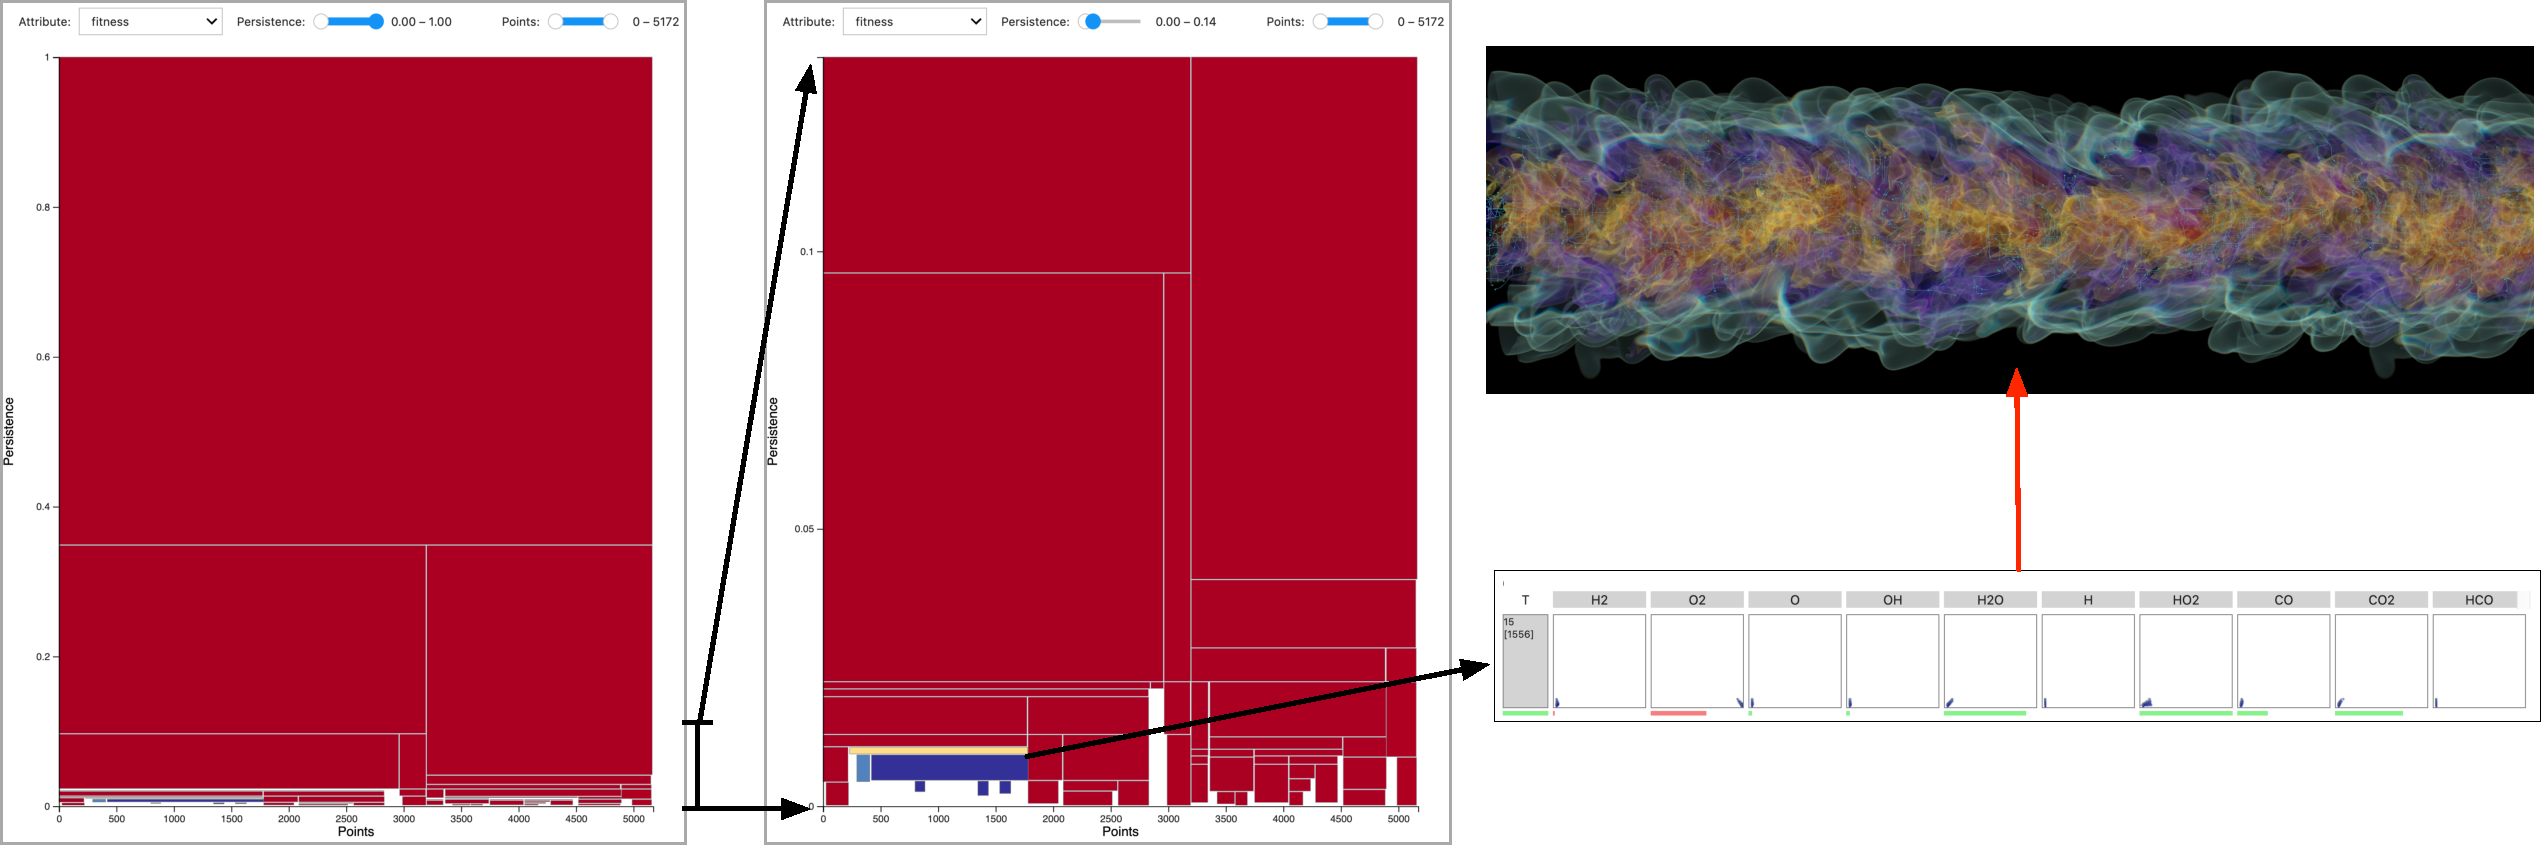
\includegraphics[width=\linewidth]{combustion-init-2}
     \vspace{-.2in}
    \caption{Combustion: Initial tree (left) shows that a single linear model describes all the data points(score = 0.998). Right: a zoom to persistence range [0:0.15] reveal a previously unknown partition containing large number (~30\%) of sample points that are outside of the active combustion zone and should have been removed (top).}
    \label{fig:combustion-init}
    \end{center}
         \vspace{-.1in}
\end{figure}

Using child and parent fitness doesn't reveal much but once we switch to child dimension fitness the tree comes to life, \autoref{fig:teaser}. The figure also shows the data points of the (four) top-most partitions that are different than their parents. Partition 494 (right most in the tree, bottom in the grid) is distinctly different from the other partitions. The three other partitions  differ mainly with respect of HO2, though the points in the first and third partitions (5 and 488) are mostly in the lower value. \autoref{fig:combustion-projections} shows the critical points graph. Note that the edges for the first three partitions overlap in (b) but are clearly separated in (c). 

The four partitions share a single maxima but feature four distinct minima. The minima in partition 494 captures a situation where fuel (H2 and CO) is available but the lack of oxidizer (O2) prevents a chemical reaction. The situation is reversed in partition 5 where oxidizer (O2) is available but the lack of fuel prevents a reaction. In partitions 460 and 488, the mixing of fuel and oxidizer is highly turbulent and blows the flames out, resulting in large amount of HO2. The clear separation between these two minima could be due to undersampling or possible the boundary of the manifold. 

% Originally only two minima were known and the third was discovered in an earlier work. The black annotation curve in (d) marks a possible boundary of the manifold, which may explain the three distinct minima we find in this area. The notches in this boundary, however, could also be due to undersampling. In contrast to the earlier work where the third minima was discovered after an exhaustive search through many potential simplifications and possible partitions, we were able to discover all four minima after a just a few steps in addition to identifying the invalid points. 

\begin{figure}[tb]
    \begin{center}
     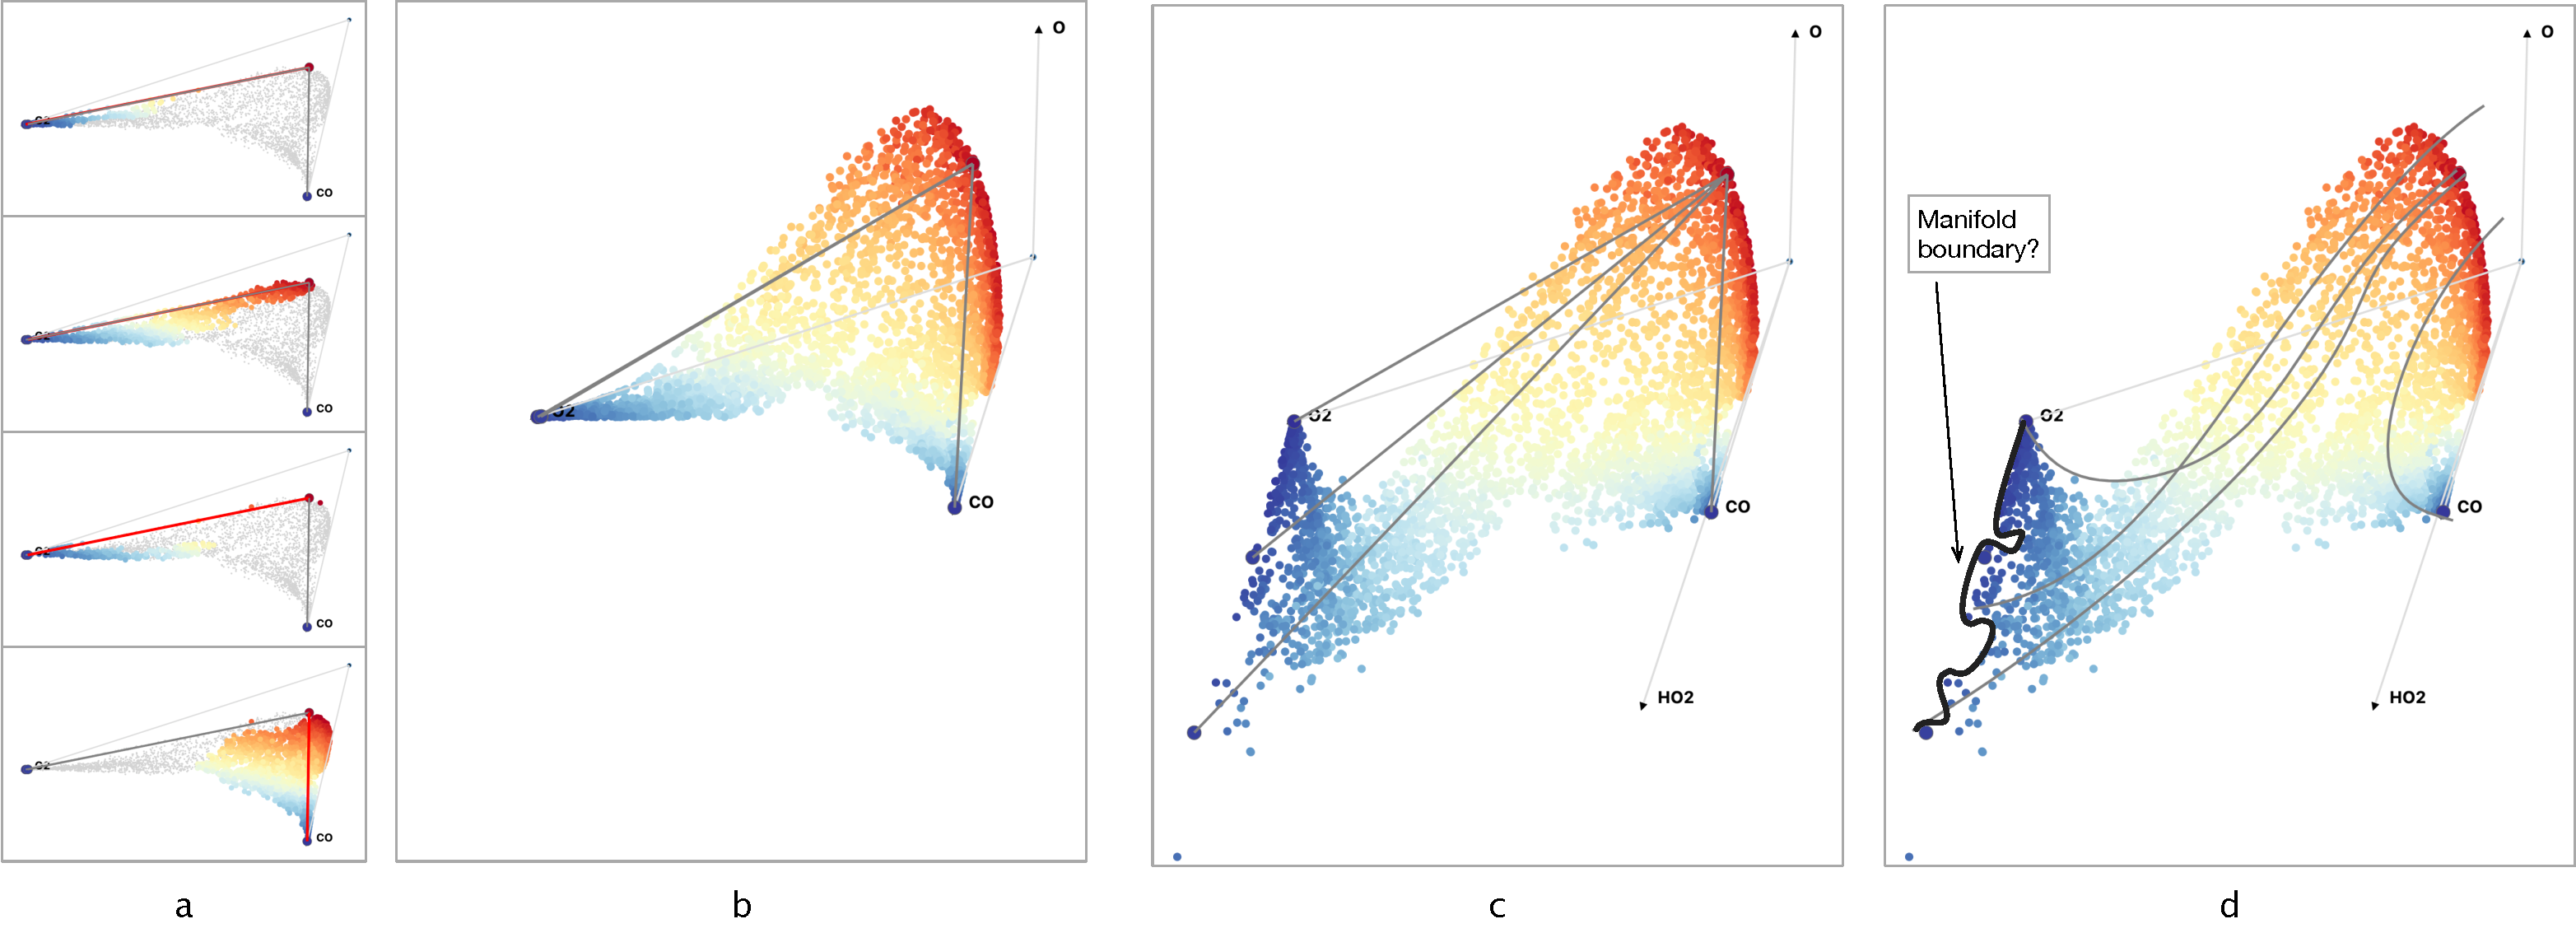
\includegraphics[width=\linewidth]{combustion-projections2}
             \vspace{-.1in}
    \caption{Graph views of the combustion data. a) Highlighting the points of each partition. b) Without the HO2 only the two expected minima are apparent. c) The three minima separates along the HO2 direction. d) Regression curves follow the shape of the manifold.}
    \label{fig:combustion-projections}
         \vspace{-.1in}
         \end{center}
\end{figure}

\subsection{Nuclear Fuel Cycle Simulations}
\label{sec:nuclear}
Nuclear fuel cycle analysis focuses on modeling the nuclear industry and ecosystem at a macroscopic level. This example studies scenarios for transitioning from one technology, Light Water Reactors (LWR) to a newer Sodium-cooled Fast breeder Reactor (SFR) technology. LWR reactors can use either enriched uranium (UOX, Uranium Oxyde) or a mixture of Uranium and Plutonium (MOX, Mixed Oxyde) as fuel but produce Minor Actinides waste. Minor Actinides have a long lifetime and high activities, which make such wastes  difficult to deal with. In contrast, SFR reactors mainly use a mix of Natural Uranium and Plutonium as a fuel (MOX). The SFR reactors have the ability to breed Plutonium from the Uranium and energy production is based on the fission of the Plutonium. This breeding capability allows the fuel to stay longer in the fuel, reducing the amount of Minor Actinides ultimately present in the waste. Some combination of fuel and SFR reactor configuration allows to breed more Plutonium than it will burn . A sufficiently large number of SFR reactors (used in 'breeder' configuration) can thus be self sustained.

\begin{figure}[b]
    \begin{center}
     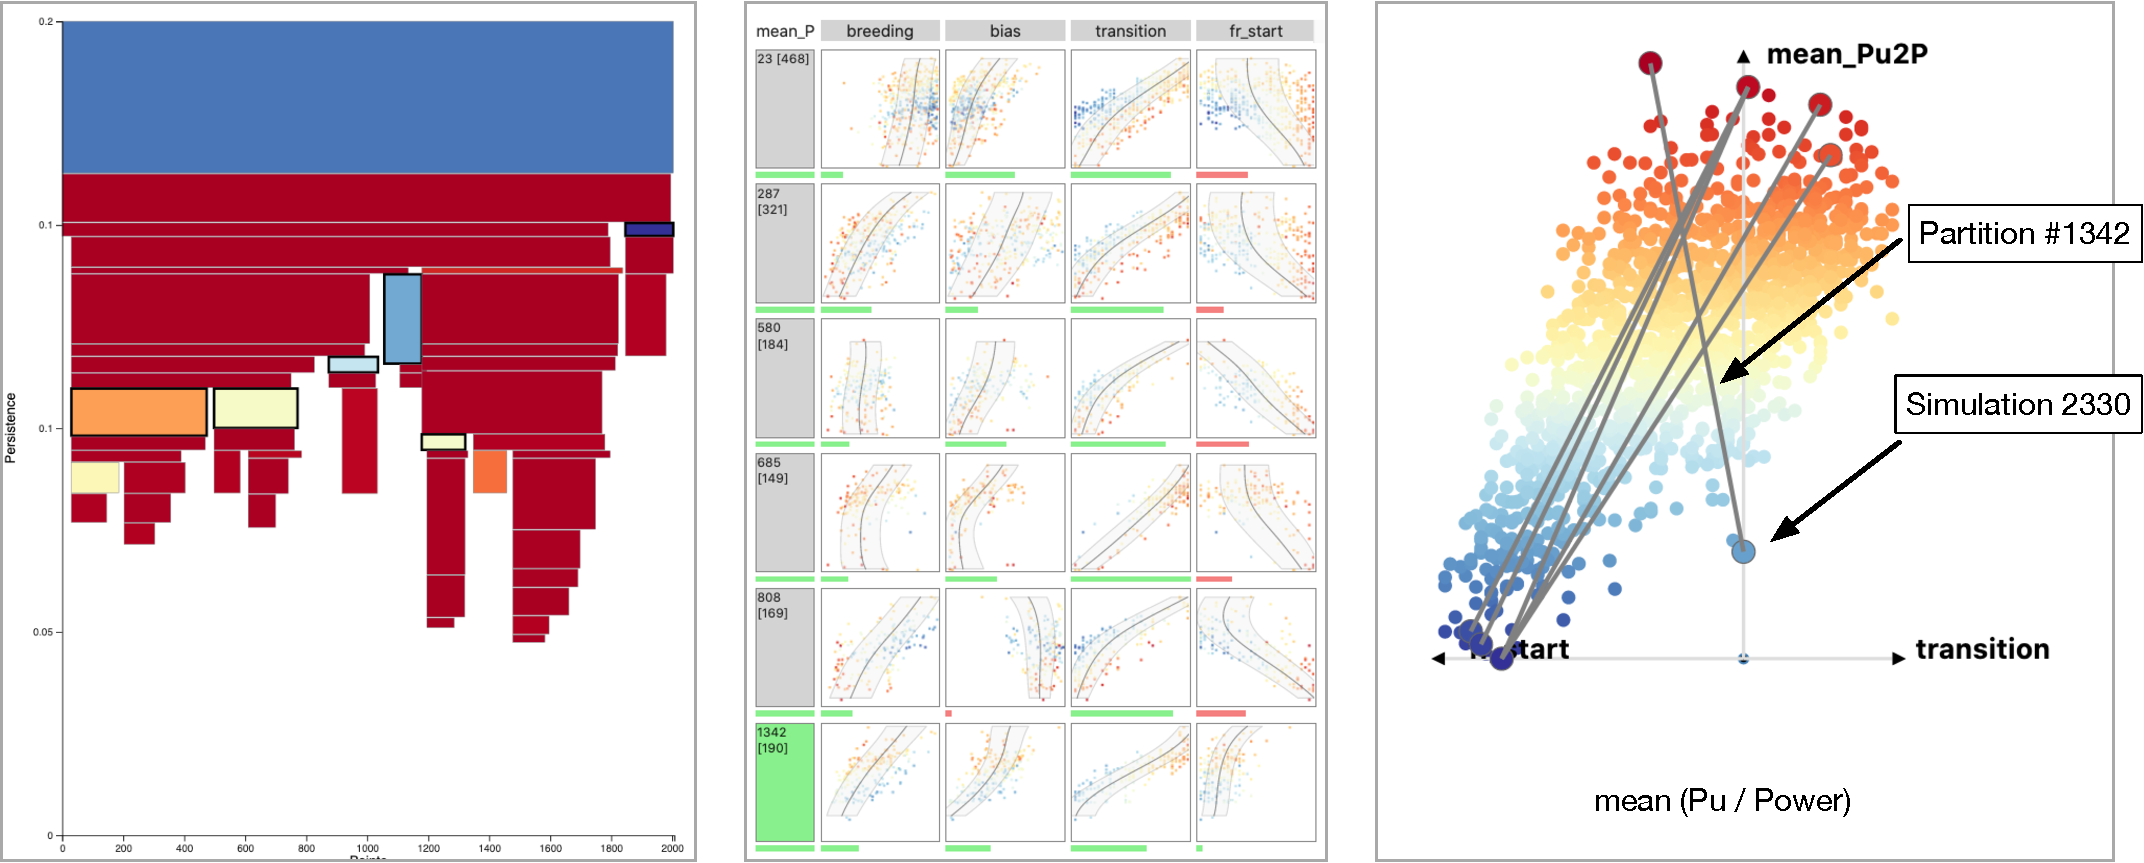
\includegraphics[width=\linewidth]{transition1}
    \caption{Transition scenario: Partitions selected based on dimension fitness (left). Partition 1342 exhibits unique behaviour (mid and right) though its minimum (simulation 2330) is not the lowest (right).}
        \vspace{-.1in}
    \label{fig:transition}
    \end{center}
\end{figure}

\begin{figure}[tb]
    \begin{center}
    \vspace{-.1in}
     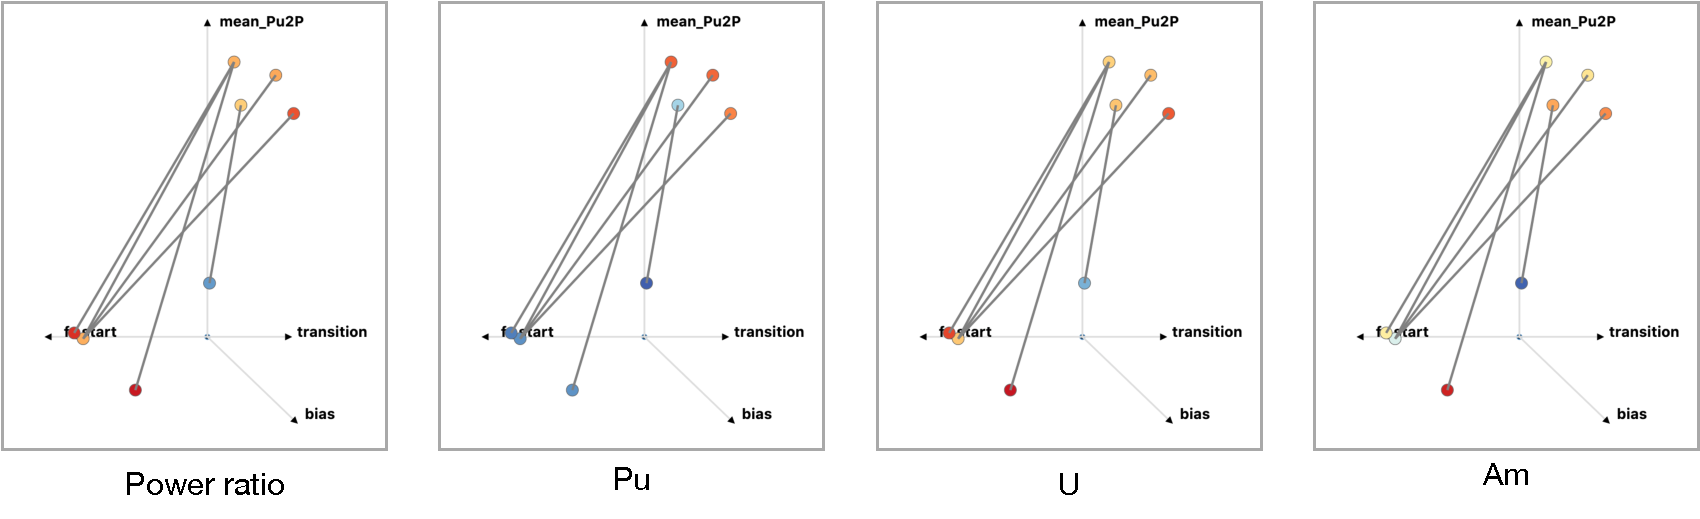
\includegraphics[width=\linewidth]{transition-graph1}
    \caption{Encoding other output variables as color demonstrates the advantages of simulation 2330 which exhibits low power ration and consistently generates low volumes of excess radio active materials.}
    \label{fig:transition-graph}
    \end{center}
\end{figure}

\begin{figure}[tb]
    \begin{center}
     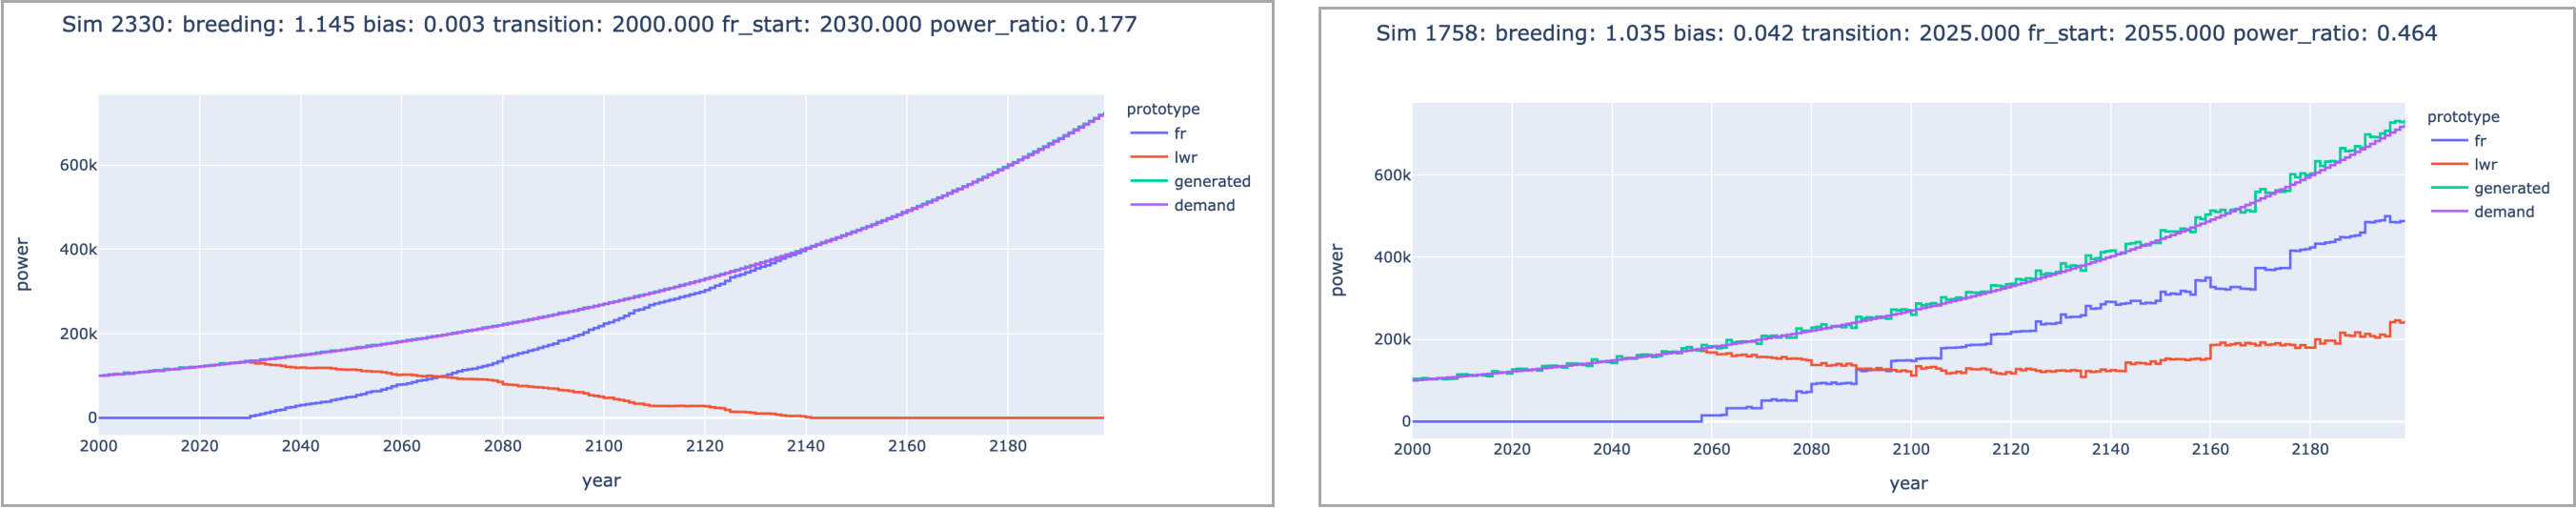
\includegraphics[width=\linewidth]{transition-plots-1}
    \caption{Simulation 2330 exhibits an excellent and smooth transition (left), while simulation 1758 does not lead to a transition (right).}
    \label{fig:transition-plots}
    \end{center}
\end{figure}

The study consists of 3300 simulation runs, using four input parameters (breeding ratio, start year of LWR fuel reprocessing, first year an SFR can be deploy and a bias measure). The aim here is to find a deployment schedule that transitions from an ecosystem consisting of LWRs to one with only SFR reactors, while minimizing some objective function. To this end we computed several objective functions at the end of each simulation including: the ratio of total power generated by LWRs reactors to the total energy generated over the simulation's 200 years span, the mean ratio of plutonium to generated power, and amount of nuclear waste such as Plutonium, Uranium and Americium. 
Of the 3300 simulation only 2007 led to a complete transition within the first 120 years). In the following we looked at the mean ration of Plutonium to power objective function. \autoref{fig:transition} show a reduced \RT (remove partitions with less than 100 simulations or a lifespan less then 0.001) depicting child dimension fitness. Several partitions that stand out are also shown. The graph view on the right shows that partition 1342 exhibits a unique behaviour, although its minima (simulation run 2330) doesn't have the lower value. \autoref{fig:transition-graph} shows that adding 'bias' in the graph view affects only one of the minima. However, when we use the same partitions and graph, but change the colors to encode other output values, we can see that simulation 2330 is unique in that it consistently exhibits low values (blues) for power ration and the amount of the nuclear waste generated. \autoref{fig:transition-plots} shows the deployment schedule of simulation 2330 (top) and an example of a simulation that doesn't lead to a complete transition. 
 


% \todo[inline]{Linear models in multi-dimensional may not be intuitive, for example the fr\_start in the transition use-case}